% Figure 2 of "The architecture of blockchain value: capabilities, pillars, and growth dynamics"
% (Papadogiannis, 2026, Front. Blockchain 9:1747512). Drawing code as in the author's manuscript.
% Compile with: pdflatex fig2_capabilities_pillars.tex
\documentclass[border=6pt]{standalone}
\usepackage{amsmath, amssymb}
\usepackage{tikz}
\usetikzlibrary{positioning, shapes, arrows.meta, calc, backgrounds}
\begin{document}
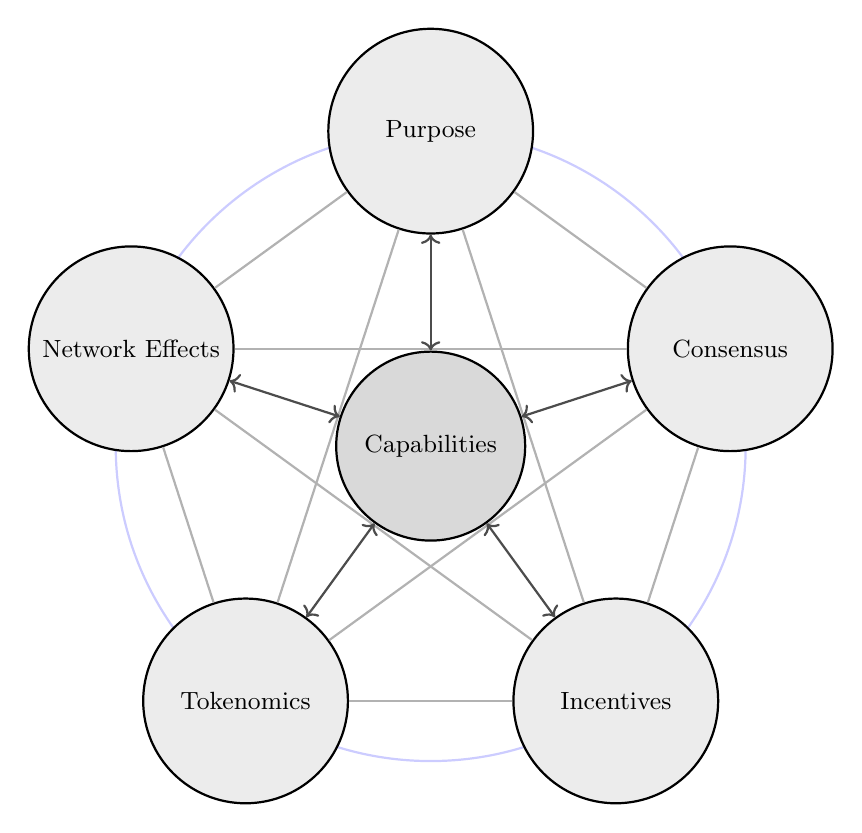
\begin{tikzpicture}[
    pillar/.style={circle, draw=black, thick, fill=gray!15, minimum size=2.6cm, align=center, font=\small},
    center/.style={circle, draw=black, thick, fill=gray!30, minimum size=2.4cm, align=center, font=\small},
    connect/.style={draw=black!30, thick},
    bidir/.style={<->, draw=black!70, thick}
]

% Light circular guide
\draw[blue!20, thick] (0,0) circle (4);

% Central node
\node[center] (capabilities) at (0,0) {Capabilities};

% Five pillars around
\node[pillar] (purpose) at (90:4) {Purpose};
\node[pillar] (consensus) at (18:4) {Consensus};
\node[pillar] (incentives) at (306:4) {Incentives};
\node[pillar] (tokenomics) at (234:4) {Tokenomics};
\node[pillar] (network) at (162:4) {Network Effects};

% Connect neighboring pillars
\draw[connect] (purpose) -- (consensus);
\draw[connect] (consensus) -- (incentives);
\draw[connect] (incentives) -- (tokenomics);
\draw[connect] (tokenomics) -- (network);
\draw[connect] (network) -- (purpose);

% Connect non-neighboring pillars
\draw[connect] (purpose) -- (incentives);
\draw[connect] (purpose) -- (tokenomics);
\draw[connect] (consensus) -- (tokenomics);
\draw[connect] (consensus) -- (network);
\draw[connect] (incentives) -- (network);

% Bidirectional arrows center → pillars
\foreach \pillar in {purpose, consensus, incentives, tokenomics, network} {
    \draw[bidir] (capabilities) -- (\pillar);
}

\end{tikzpicture}
\end{document}
